\chapter{\textit{Backtracking}}
\thispagestyle{chapterInit}

Il \textit{backtracking} è una tecnica di ricerca che consente di esplorare in modo sistematico tutte le possibili \textbf{soluzioni ammissibili} di un problema, per trovare una o più soluzioni valide. Una volta trovate tutte le soluzioni ammissibili queste vengono \textbf{valutate} per meglio risolvere i problemi di \textbf{ottimizzazione} che richiedono una soluzione ottimale. 
\begin{definition}[Soluzione ammissibile]
    Dato un problema, una \textbf{soluzione ammissibile} è una soluzione che soddisfa \textbf{un insieme di criteri} definiti per il problema stesso.
\end{definition}
\begin{definition}[Soluzione ottimale]
    Dato un problema, una \textbf{soluzione ottimale} è una soluzione ammissibile che soddisfa \textbf{un insieme di criteri} definiti per il problema stesso e che è \textbf{migliore} rispetto a tutte le altre soluzioni ammissibili.
\end{definition}
\section{\textit{Backtracking} v/s \textit{Brute Force}}
    In alcuni problemi è richiesto esplorare \textbf{l'intero spazio} delle soluzioni ammissibili, questo può essere necessario in questi casi:
    \paragraph{Problemi di enumerazione} Nei problemi di enumerazione è richiesto di trovare tutte le soluzioni ammissibili. Ad esempio, elencare tutte le permutazioni di un insieme di numeri. 
        \subparagraph{Soluzione} Usiamo degli algoritmi di enumerazione
    \paragraph{Problemi di ricerca} Nei problemi di ricerca è richiesto di trovare una o più soluzioni ammissibili. Ad esempio, trovare una sequenza di mosse per il gioco del 15. 
        \subparagraph{Soluzione} Usiamo degli algoritmi enumerazione e ci fermiamo alla prima soluzione trovata.
    \paragraph{Problemi di conteggio} Nei problemi di conteggio è richiesto di contare il numero di soluzioni ammissibili. Ad esempio, contare il numero di possibilità che esistono di esprimere un numero $n$ come somma di $k$ numeri primi.
        \subparagraph{Soluzione} Se il conteggio analitico non è possibile, usiamo degli algoritmi di enumerazione andando a trovare tutte le soluzioni ammissibili e contando il numero di soluzioni trovate.
    \paragraph{Problemi di ottimizzazione} Nei problemi di ottimizzazione è richiesto di trovare la soluzione ammissibile migliore rispetto ad un criterio definito. Trovare il cammino di peso massimo in un grafo dal punto $A$ al punto $B$.
        \subparagraph{Soluzione} Enumeriamo tutti i cammini ammissibili e calcoliamo il peso di ciascuno di essi. La soluzione ottimale è il cammino con peso massimo.
    \subsubsection{Il costo}
        Per tutte queste soluzioni abbiamo dovuto analizzare e calcolare l'intero spazio delle possibili soluzioni che possono anche avere una dimensione super-polinomiale, talvolta questa è l'unica strada per risolvere il problema. Per problemi di dimensione medio-piccoli non è un problema, ma per problemi di dimensione grande il costo di calcolo diventa inaccettabile. Per alcuni di questi problemi non deve essere necessariamente calcolato l'intero spazio delle soluzioni ammissibili, ma solo una parte di esso. 
    \subsubsection{\textit{Backtracking}}
        La filosofia del \textit{backtracking} è quella di esplorare lo spazio delle soluzioni in modo sistematico, se ad un certo punto si scopre che una soluzione non è ammissibile, si torna indietro e si esplora un'altra soluzione. In questo modo si evita di esplorare l'intero spazio delle soluzioni, ma si esplora solo una parte di esso andando ad eliminare le soluzioni che non sono ammissibili.
        \paragraph{Ricorsione} Grazie alla ricorsione possiamo sistematicamente esplorare uno spazio di ricerca ed memorizzare le soluzioni parziali.
        \paragraph{Iterazione} In alcuni casi è possibile utilizzare un approccio iterativo \textit{greedy} per risolvere il problema. Questa strategia può essere utile negli inviluppi convessi o nello \textit{string matching}.
\section{Enumerazione}
    Ora prendiamo in considerazione i problemi di enumerazione, in cui è richiesto di trovare tutte le soluzioni ammissibili. In questo caso il \textit{backtracking} può essere utilizzato per generare tutte le soluzioni ammissibili in modo sistematico.
    \subsubsection{Organizzazione Generale}
        Generalmente una soluzione è rappresenta da un vettore di scelte: $S[1\dots n]$ dove $S[i]$ è la scelta fatta per il passo $i$ presa da un insieme di scelte $C$ \textbf{dipendente} dal problema.
    \subsubsection{Soluzioni Parziali}
        Una soluzione parziale è una soluzione che non è completa, ma sono già state fatte scelte fino ad $i$ ed la nostra soluzione $S[1\dots i-1]$ contiene le scelte fatte fino ad ora. Ora se $S[1\dots i-1]$ è una soluzione ammissibile allora la processiamo assumendo che questa non possa essere estesa. Se invece $S[1\dots i-1]$ non è una soluzione ammissibile, allora calcoliamo l'insieme di scelte $C$ per il passo $i$ e per ogni scelta $c \in C$ proviamo ad estendere la soluzione parziale $S[1\dots i-1]$ con la scelta $c$. Eseguiamo dunque la ricorsione per il passo $i+1$ e continuiamo fino a quando non abbiamo esaurito tutte le scelte. Se una scelta non porta ad una soluzione ammissibile, torniamo indietro e proviamo un'altra scelta. Questo processo continua fino a quando non abbiamo trovato tutte le soluzioni ammissibili.\newline
        Per rappresentare queste scelte è possibile usare un \textbf{albero delle decisioni} che corrisponde allo spazio di ricerca, la radice è la soluzione parziale vuota, per ogni nodo c'è un passo $i$ e per ogni figlio c'è una scelta $c \in C$. Ogni foglia corrisponde ad una soluzione ammissibile.
    \newpage
    \subsection{Sottoinsiemi e Permutazioni}
        \subsubsection{Sottoinsiemi}
            Elencare tutti i sottoinsiemi dell'insieme $S = \{1,\dots, n\}$.\newline
            Sarà dunque possibile scrivere i seguenti algoritmi:
            \begin{algorithm}[H]
                \caption{\textsc{subsetsRec}(\Int $n$, \Int[] $S$, \Int $i$)}
                \begin{algorithmic}
                    \If{$i > n$} \Comment{$S$ ammissibile dopo $n$ scelte}
                        \State \Call{processSolution}{$S, n$}
                    \Else \Comment{Eseguiamo la scelta di prendere o non prendere l'elemento $i$}
                        \State \Set $C \gets \{0, 1\}$
                        \For{$c \in C$}
                            \State $S[i] \gets c$
                            \State \Call{subsetsRec}{$n, S, i + 1$}
                        \EndFor
                    \EndIf
                \end{algorithmic}
            \end{algorithm}
            La chiamata iniziale sarà: 
            \begin{algorithm}[H]
                \caption{\textsc{subsets}(\Int $n$)}
                \begin{algorithmic}
                    \State \Int$[]$ $S \gets \New \Int[1\dots n]$
                    \State \Call{subsetsRec}{$n, S, 1$}
                \end{algorithmic}
            \end{algorithm}
            Ed infine la funzione per processare la soluzione:
            \begin{algorithm}[H]
                \caption{\textsc{processSolution}(\Int[] $S$, \Int $n$)}
                \begin{algorithmic}
                    \State \Call{print}{"\{ "}
                    \For{$i \gets 1$ \textbf{to} $n$}
                        \If{$S[i] = 1$}
                            \State \Call{print}{$i$, " "}
                        \EndIf
                    \EndFor
                    \State \Call{println}{"\}"}
                \end{algorithmic}
            \end{algorithm}
            \paragraph{Complessità} La complessità di questo algoritmo è $\Theta(n\cdot 2^n)$ perché ci sono $2^n$ sottoinsiemi e per ognuno di essi dobbiamo stampare al massimo $n$ elementi. La rappresentazione come albero delle decisioni per $n = 3$ è la seguente:
            \begin{figure}[H]
                \centering
                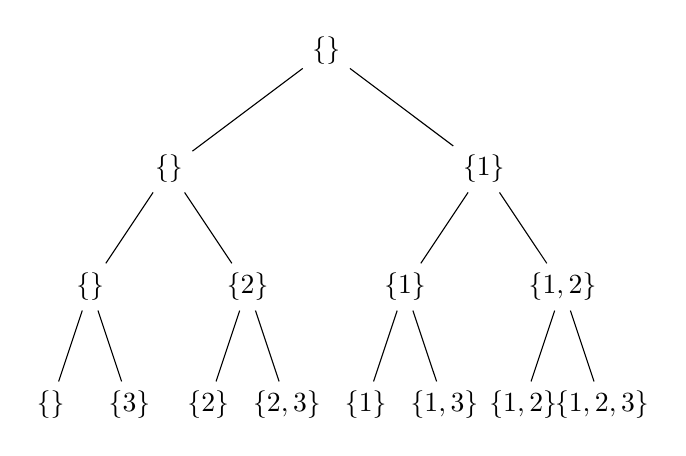
\begin{tikzpicture}
                    \node(0){$\{\}$}
                        [sibling distance=4cm]
                        child{node{$\{\}$}
                            [sibling distance=2cm]
                            child{node{$\{\}$}
                                [sibling distance=1cm]
                                child{node{$\{\}$}}
                                child{node{$\{3\}$}}
                            }
                            child{node{$\{2\}$}
                                [sibling distance=1cm]
                                child{node{$\{2\}$}}
                                child{node{$\{2,3\}$}}
                            }
                        }
                        child{node{$\{1\}$}
                            [sibling distance=2cm]
                            child{node{$\{1\}$}
                                [sibling distance=1cm]
                                child{node{$\{1\}$}}
                                child{node{$\{1,3\}$}}
                            }
                            child{node{$\{1,2\}$}
                                [sibling distance=1cm]
                                child{node{$\{1,2\}$}}
                                child{node{$\{1,2,3\}$}}
                            }
                        };
                \end{tikzpicture}
                \caption{Albero delle decisioni per $n = 3$}
            \end{figure}
            Esiste la versione iterativa per la risoluzione di questo problema? Si ed il costo è $\Theta(n\cdot 2^n)$
            \begin{algorithm}[H]
                \caption{\textsc{subsetsIter}(\Int $n$)}
                \begin{algorithmic}
                    \For{$j \gets 0$ \To $2^n - 1$}
                        \State \Call{print}{"\{ "}
                        \For{$i \gets 0$ \To $n - 1$}
                            \If{$j \&\& 2^i \neq 0$} \Comment{\textit{Bitwise and}}
                                \State \Call{print}{$i$, " "}
                            \EndIf
                        \EndFor
                        \State \Call{println}{"\}"}
                    \EndFor
                \end{algorithmic}
            \end{algorithm}
            La complessità visto il primo ciclo da $0$ a $2^n - 1$ ed il ciclo interno da $0$ a $n - 1$ è $\Theta(n\cdot 2^n)$.
        \subsubsection{Permutazioni}
            Elencare tutte le permutazioni dell'insieme $S = \{1,\dots, n\}$.\newline
            Sarà dunque possibile scrivere i seguenti algoritmi:
            \begin{algorithm}[H]
                \caption{\textsc{permutationsRec}(\Set $A$, \Item[] $S$, \Int $i$)}
                \begin{algorithmic}
                    \If{$A.\Call{isEmpty}{}$} \Comment{Tutte le scelte sono state fatte}
                        \State \Call{print}{$S$}
                    \Else \Comment{Eseguiamo la scelta di prendere o non prendere l'elemento $i$}
                        \Set $C \gets A.\Call{copy}{}$
                        \ForEach{$c \in C$}
                            \State $S[i] \gets c$
                            \State $A.\Call{remove}{c}$
                            \State \Call{permutationsRec}{$A, S, i + 1$}
                            \State $A.\Call{insert}{c}$
                        \EndFor
                    \EndIf
                \end{algorithmic}
            \end{algorithm}
            La chiamata iniziale sarà:
            \begin{algorithm}[H]
                \caption{\textsc{permutations}(\Set $A$)}
                \begin{algorithmic}
                    \State \Int $n \gets A.\Call{size}()$
                    \State \Item[] $S \gets \New \Item[1\dots n]$
                    \State \Call{permutationsRec}{$A, S, 1$}
                \end{algorithmic}
            \end{algorithm}
            In questo caso l'albero delle decisioni è:
            \begin{figure}[H]
                \centering
                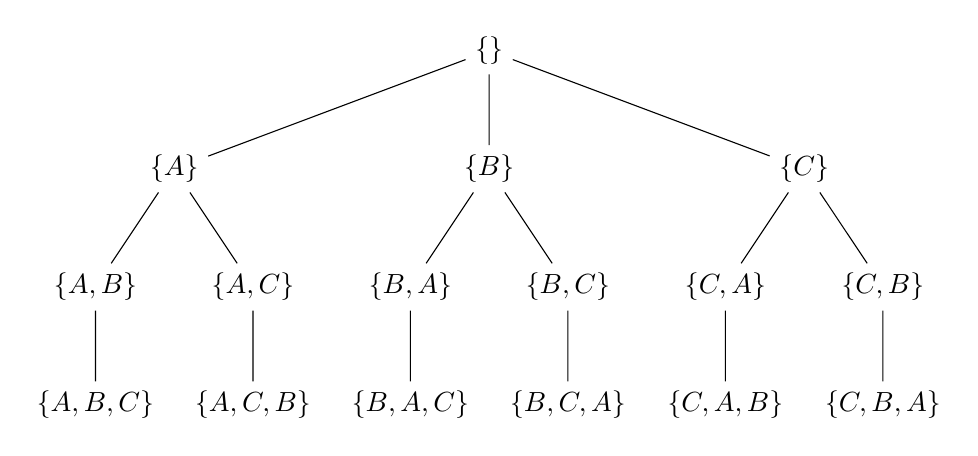
\begin{tikzpicture}
                    \node(0){$\{\}$}
                        [sibling distance=4cm]
                        child{node{$\{A\}$}
                            [sibling distance=2cm]
                            child{node{$\{A, B\}$}
                                [sibling distance=1cm]
                                child{node{$\{A, B, C\}$}}
                            }
                            child{node{$\{A, C\}$}
                                [sibling distance=1cm]
                                child{node{$\{A, C, B\}$}}
                            }
                        }
                        child{node{$\{B\}$}
                            [sibling distance=2cm]
                            child{node{$\{B, A\}$}
                                [sibling distance=1cm]
                                child{node{$\{B, A, C\}$}}
                            }
                            child{node{$\{B, C\}$}
                                [sibling distance=1cm]
                                child{node{$\{B, C, A\}$}}
                            }
                        }
                        child{node{$\{C\}$}
                            [sibling distance=2cm]
                            child{node{$\{C, A\}$}
                                [sibling distance=1cm]
                                child{node{$\{C, A, B\}$}}
                            }
                            child{node{$\{C, B\}$}
                                [sibling distance=1cm]
                                child{node{$\{C, B, A\}$}}
                            }
                        };
                \end{tikzpicture}
                \caption{Albero delle decisioni per $n = 3$}
            \end{figure}
            \paragraph{Complessità} La complessità di questo algoritmo è $\Theta(n\cdot n!)$ in quanto la stampa di ogni permutazione richiede $O(n)$, il costo delle copie richieste per ogni permutazione è $\sum_{1}^{n} O(i) = O(n^2)$ e il numero di foglie è $n!$, dunque il costo totale è $O(n^2 \cdot n!)$.
            \paragraph{Soluzione alternativa} Questo enorme costo può essere ridotto a $\Theta(n \cdot n!)$ se evitiamo di copiare l'insieme $A$ ad ogni passo. In questo caso usando lo stesso vettore andremo a scambiare l'elemento corrente con l'elemento $i$ e eseguiremo la ricorsione. Al termine della ricorsione andremo a scambiare nuovamente l'elemento corrente con l'elemento $i$ per ripristinare lo stato iniziale ed eseguire le chiamate ricorsive ``sorelle'' a quella eseguita.
            \begin{algorithm}[H]
                \caption{\textsc{permutationsRec}(\Item[] $S$, \Int $i$)}
                \begin{algorithmic}
                    \If{$i == 1$} \Comment{Tutte le scelte sono state fatte}
                        \State \Call{println}{$S$}
                    \Else
                        \For{$j \gets 1$ \To $i$}
                            \State \Call{swap}{$S, i, j$}
                            \State \Call{permutationsRec}{$S, i - 1$}
                            \State \Call{swap}{$S, i, j$} \Comment{Ripristina lo stato iniziale}
                        \EndFor
                    \EndIf
                \end{algorithmic}
            \end{algorithm}
            \paragraph{Complessità} La complessità di questo algoritmo è $\Theta(n \cdot n!)$ in quanto la stampa di ogni permutazione richiede $O(n)$ e il numero di foglie è $n!$ e non abbiamo più il costo delle copie richieste per ogni permutazione. Il costo totale è dunque $O(n \cdot n!)$.
        \subsubsection{Schema completo enumerazione}
            Per risolvere i problemi di enumerazione è possibile la seguente ``base'' come algoritmo generale di enumerazione:
            \begin{algorithm}[H]
                \caption{\textsc{enumerate}($\left<\text{dati problema}\right>, \Item[] S, \Int i, \left<\text{dati parziali}\right>$)}
                \begin{algorithmic}
                    \If{\Call{accept}{$\left<\text{dati problema}\right>, S, i, \left<\text{dati parziali}\right>$}} \Comment{Controlla se la soluzione è ammissibile}
                        \State \Call{processSolution}{$\left<\text{dati problema}\right>, S, i, \left<\text{dati parziali}\right>$} \Comment{Processa la soluzione ammissibile}
                    \ElsIf{\Call{reject}{$\left<\text{dati problema}\right>, S, i, \left<\text{dati parziali}\right>$}} \Comment{Controlla se la soluzione è da scartare}
                        \State \Return \Comment{Scarta la soluzione}
                    \Else \Comment{Eseguiamo una scelta}
                        \State \Set $C = \Call{choices}{\left<\text{dati problema}\right>, S, i, \left<\text{dati parziali}\right>}$ \Comment{Calcola le scelte}
                        \ForEach{$c \in C$} \Comment{Per ogni scelta}
                            \State $S[i] \gets c$ \Comment{Aggiorna la soluzione parziale}
                            \State \Call{enumerate}{$\left<\text{dati problema}\right>, S, i + 1, \left<\text{dati parziali}\right>$} \Comment{Esegui la ricorsione}
                        \EndFor
                    \EndIf
                \end{algorithmic}
            \end{algorithm}
            Notiamo come rispetto allo schema generale di \textit{backtracking} abbiamo aggiunto la parte di rifiuto della soluzione. Questa ci permette di scartare delle possibili strade se si scopre che proseguendo con le scelte non si arriverà mai ad una soluzione ammissibile. Nota come nei casi precedenti non possiamo mai scartare una soluzione, ma dobbiamo sempre esplorare l'intero spazio delle soluzioni ammissibili.
        \subsubsection{$k$-Sottoinsiemi}
            Dato un insieme $S$ di $n$ elementi, elencare tutti i sottoinsiemi di $k$ elementi.\newline
            Una prima idea è quella di non prendere in considerazione le soluzioni se alla fine non abbiamo $k$ elementi. In questo caso analizziamo comunque l'intero spazio delle soluzioni ammissibili.\newline
            Un ulteriore miglioramento è quello di scartare tutte le soluzioni che dopo $i$ scelte abbiano lo stesso numero di $k$ elementi o superiori. In questo caso possiamo scartare tutte quelle soluzioni sicuramente inammissibili in quanto avranno un numero di elementi maggiore di $k$.\newline
            Infine possiamo scartare anche le soluzioni parziali che, anche se dalla scelta $i$ in poi prendessero tutti gli elementi, non arriverebbero a $k$ elementi ($n-(i-1)<missing$). In questo caso possiamo scartare tutte quelle soluzioni sicuramente inammissibili in quanto avranno sicuramente un numero di elementi minore di $k$.\newline
            Alla fine dei miglioramenti (\textit{pruning}) il nostro algoritmo sarà:
            \begin{algorithm}[H]
                \caption{\textsc{kSubsetsRec}(\Int $n$, \Int $missing$, \Int[] $S$, \Int $i$)}
                \begin{algorithmic}
                    \If{$missing == 0$} \Comment{Tutte le scelte sono state fatte}
                        \State \Call{processSolution}{$S, i-1$}
                    \ElsIf{$i\leq n \And 0 < missing \leq n - i + 1$} \Comment{Eseguiamo la scelta di prendere o non prendere l'elemento $i$}
                        \ForEach{$c\in\{ 0,1\}$}
                            \State $S[i] \gets c$ \Comment{Aggiorna la soluzione parziale}
                            \State \Call{kSubsetsRec}{$n, missing - c, S, i + 1$} \Comment{Vado avanti con la ricorsione}
                        \EndFor
                    \EndIf
                \end{algorithmic}
            \end{algorithm}
            L'albero delle decisioni per $n = 4$ e $k = 2$ dopo aver applicato il \textit{pruning} è:
            \begin{figure}[H]
                \centering
                \begin{tikzpicture}
                    \node(0){$\{\}$}
                        [sibling distance=8cm]
                        child{node{$\{\}$}
                            [sibling distance=4cm]
                            child{node{$\{\}$}
                                [sibling distance=2cm]
                                child{node{$\{\}$}}
                                child{node{$\{3\}$}
                                    [sibling distance=1cm]
                                    child{node{$\{3\}$}}
                                    child{node{$\{3,4\}$}}
                                }
                            }
                            child{node{$\{2\}$}
                                [sibling distance=2cm]
                                child{node{$\{2\}$}
                                    [sibling distance=1cm]
                                    child{node{$\{2\}$}}
                                    child{node{$\{2,4\}$}}
                                }
                                child{node{$\{2,3\}$}}
                            }
                        }
                        child{node{$\{1\}$}
                            [sibling distance=4cm]
                            child{node{$\{1\}$}
                                [sibling distance=2cm]
                                child{node{$\{1\}$}
                                    [sibling distance=1cm]
                                    child{node{$\{1\}$}}
                                    child{node{$\{1,4\}$}}
                                }
                                child{node{$\{1,2\}$}}
                            }
                            child{node{$\{1,3\}$}}
                        };
                \end{tikzpicture}
                \caption{Albero delle decisioni per $n = 4$ e $k = 2$}
            \end{figure}
        \subsubsection{Ricapitolando}
            Quando specializziamo un algoritmo di \textit{backtracking} per un problema specifico, dobbiamo valutare la possibilità di eseguire del \textit{pruning} per evitare di esplorare soluzioni che non possono mai essere ammissibili. Spesso la versione con \textit{pruning} è più efficiente per valori di $k$ piccoli o grandi, ma non lo sarà altrettanto per valori intermedi, comunque anche per quest'ultimi sarà possibile apprezzare un miglioramento rispetto alla versione senza \textit{pruning}. \newline
            In questo caso non è possibile ottenere lo stesso risultato con un algoritmo iterativo, in quanto non è possibile scartare le soluzioni parziali che non portano a soluzioni ammissibili. 
    \subsection{\textit{Subset sum} - Somma di sottoinsieme}
        Il problema prevede che dato un vettore $A$ contenente $n$ interi positivi, ed un intero positivo $k$ di trovare, se esiste, un sottoinsieme $S\subseteq \{1\dots n\}$ tale che $\sum_{i\in S}a[i]=k$?
        \subsubsection{Analisi del problema}
            Grazie al \textit{backtracking} lo risolveremmo in $O(2^n)$ dovendo analizzare ogni elemento del vettore $A$ e decidere se includerlo o meno nel sottoinsieme $S$.\newline
            In programmazione dinamica può essere risolto in $O(n\cdot k)$, ma non è sempre possibile. Che è pseudo-polinomiale, in quanto il costo dipende da $k$ e da $n$.\newline
            Però per lo scopo del problema a noi non interessano tutte le soluzioni ma solo una, se esiste, quindi nel momento in cui troviamo una soluzione ammissibile possiamo interrompere l'algoritmo.
        \subsubsection{Soluzione}
            Andiamo allora a specializzare l'algoritmo di \textit{backtracking} con \textit{pruning} per evitare di esplorare soluzioni che non possono mai essere ammissibili. 
            \begin{algorithm}[H]
                \caption{\Bool \textsc{subsetSumRec}(\Int[] $A$, \Int $n$, \Int $missing$, \Int[] $S$, \Int $i$)}
                \begin{algorithmic}
                    \If{$missing == 0$} \Comment{Tutte le scelte sono state fatte}
                        \State \Call{processSolution}{$S, i-1$}
                        \State \Return \True
                    \ElsIf{$i>n \Or missing < 0$} \Comment{Controlla se la soluzione è da scartare}
                        \State \Return \False
                    \Else \Comment{Eseguiamo una scelta}
                        \State \Set $C = \{ 0,1\}$
                        \ForEach{$c\in C$}
                            \State $S[i] \gets c$ \Comment{Aggiorna la soluzione parziale}
                            \If{\Call{subsetSumRec}{$A, n, missing - A[i]\cdot c, S, i + 1$}}
                                \State \Return \True
                            \EndIf
                        \EndFor
                        \State \Return \False
                    \EndIf
                \end{algorithmic}
            \end{algorithm}
            Se si potesse avere l'informazione sulle somme cumulative si potrebbe ridurre ancora il costo.
    